\chapter{Metodología utilizada}

Para este proyecto se ha usado metodologías ágiles basadas en SCRUM \cite{scrum}. No ha sido posible seguir SCRUM de una manera más precisa, ya que este proceso está enfocado a trabajar en
equipo, en entornos complejos y orientado a la existencia de clientes. En este caso, al ser un único desarrollador y un entorno tan complejo, el proceso basado en SCRUM se ha
focalizado más en buscar realizar entregas parciales y regulares hacia el producto final. Esto se ha llevado a cabo convirtiendo las historias de usuario en una serie de hitos
que se deben ir alcanzando para tener la historia de usuario completa.\\

\section{Planificación}

Para la planificación de este proyecto, se ha partido de historias de usuario las cuales se desean complacer. A partir de estas, se han creado una serie de hitos que conformaban productos mínimamente viables,
 que nos llevan hasta el producto final.

\subsection{Historias de usuario}

Para conseguir las historias de usuario sobre las cuales se generarán los hitos, hay que personificar tipos de usuarios que necesitan nuestra aplicación, ya que se encuentran en su día a día
con problemas los cuales se resuelven con la misma. En este caso, se parten de estas \textit{user journeys}:

\newpage

\begin{itemize}
    \item \textbf{Javier Ruiz:} Estudiante de farmacia que ha tenido que mudarse a una ciudad para estudiar, el cual cuando vuelve a su pueblo,
     se reúne con sus amigos a jugar un partido de fútbol como cuando compartían clase. Debido a que sus amigos suelen estar muy ocupados,
     no siempre están todos disponibles para jugar. Normalmente, pierden bastante tiempo en formar los equipos buscando que el partido esté igualado,
     ya que aún mantienen el pique de demostrar quien es el jugador con más nivel de la pandilla. 
    \item \textbf{Jose Muñoz} Estudiante que, cuando tiene un rato libre, le gusta juntarse con sus amigos para jugar a fútbol. En su grupo de amigos también hay otros 4 Joses, por lo que
    se vuelve un lío saber a que Jose se refieren cada vez a la hora de hacer los equipos para jugar el partido.
\end{itemize}

Y una vez tenemos el contexto en el que ocurre el problema, ya se pueden crear las \href{https://github.com/manujurado1/SportsBar-IV/labels/user-stories}{historias de usuario}:

\begin{itemize}
    \item \href{https://github.com/manujurado1/SportsBar-IV/issues/107}{Javier} quiere tener la posibilidad de crear un grupo donde estén todos sus amigos que juegan a fútbol y, indicando cuáles están disponibles para cada partido, crear 2
    equipos de fútbol igualados según el nivel alcanzado por cada jugador. Javier quiere que ese nivel no sea fijo, y pueda ir variando con el tiempo para intentar igualar
    al máximo los partidos y para poder, de alguna forma, consultar el nivel de todos sus amigos para ver quien es el mejor jugador actualmente.
    \item \href{https://github.com/manujurado1/SportsBar-IV/issues/119}{Jose} juega en un grupo de amigos donde hay otros cinco Joses. En el pasado, cuando se ha incorporado a un grupo, nunca sabía cuando salían los grupos en qué equipo estaba. A veces le ponían "Jose el nuevo", pero luego llegaba otro Jose y ya no sabía a quién se referían. Otros se ofrecían a ponerle Jose 2 o Jose 3 pero nunca se acordaba qué Jose era en qué grupo. Algunos le decían de añadir alguna característica física, pero eso le resultaba muy incómodo.
    En resumen, Jose quiere que le identifiquen por su nombre, pero si hay otras personas con el mismo nombre, quiere añadir alguna característica que sea fácilmente recordable (como la fecha de nacimiento, que no es repetible, o parte de ella) en vez de otras características que le asigne alguien (porque son difíciles de recordar) o que contengan datos personales sensibles que no tiene por qué conocer todo el grupo de amigos (como el móvil o el DNI).
    Así, cuando vea Jose de noviembre del 99 sabrá que se trata de él.
\end{itemize}

\newpage
\section{Temporización}

La temporización del proyecto se ha realizado por medio de \textit{sprints}.\\

En cada uno de estos \textit{sprints} se han ido fijando una serie de problemas a resolver, todos ellos enfocados a satisfacer las historias de usuario, avanzando en cada momento
alguno de los hitos mencionados anteriormente.


\section{Seguimiento del desarrollo}

Con el fin de obtener una mayor trazabilidad de cómo se ha ido desarrollando el proyecto, se ha usado Git como sistema de control de versiones, el cual nos permite ver versiones anteriores
del proyecto, revertir cambios y progresar en el proyecto por distintas ramas, lo que aumenta el grado de adaptabilidad.\\

Para alojar este proyecto se ha utilizado GitHub. Esta plataforma permite observar en todo momento cuál es el estado actual del proyecto y además ofrece herramientas para el control de calidad
a través de las \textit{GitHub Actions} \cite{actions}, de las que hablaremos a continuación.

\begin{figure}[H]
	\centering	
	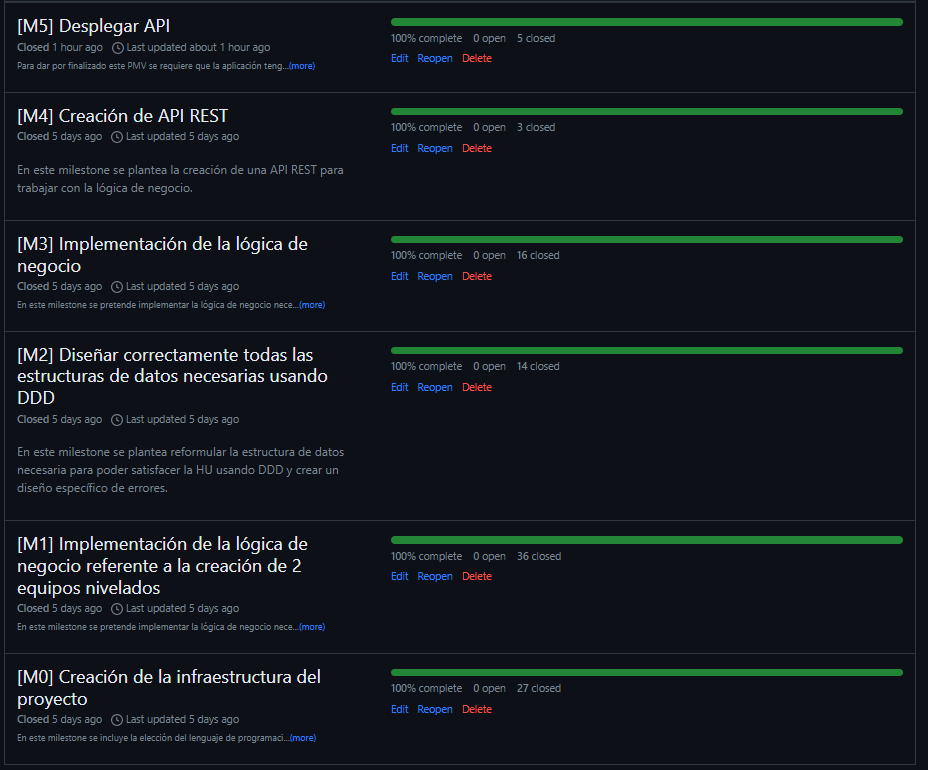
\includegraphics[scale=0.5]{img/milestones.png}
	\caption{Milestones creados en GitHub para realizar el proyecto}
\end{figure}


\section {Control de calidad}

Para dotar al proyecto de calidad se han implementado junto al desarrollo del mismo una serie de \textit{tests} siguiendo la práctica de desarrollo dirigido por pruebas o TDD.\\

Siguiendo esta práctica, se ha priorizado la creación de las pruebas, escribiendo el código fuente tras estas. De esta manera, se da el código por válido cuando este supera sus pruebas asociadas.
De esta forma se crea una batería de pruebas, la cual empieza con una base de pruebas unitarias y acaba con pruebas de integración y \textit{End-to-end}.\\

Estos controles de calidad han sido muy provechosos al fusionarlos con la integración continua, práctica de desarrollo software mediante la cuál se ejecutan pruebas automáticas sobre el código cuando este es modificado.
La integración continua se ha conseguido usando \textit{GitHub Actions}\cite{actions} y \textit{Checks API}, ambas herramientas provenientes de GitHub.

Además, se ha introducido otra \textit{GitHub Actions} que lanza un linter, en este caso golangci-lint \cite{golangci-lint} para asegurar un código fuente de calidad

\begin{figure}[H]
	\centering	
	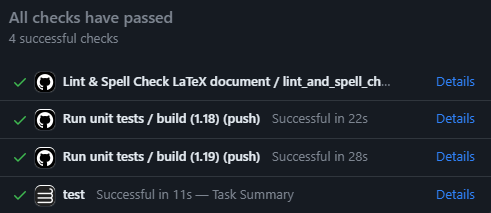
\includegraphics[scale=1]{img/actions.png}
	\caption{Ejemplo real control de calidad}
\end{figure}

\newpage